\documentclass{article}
\usepackage{amsmath}
\usepackage{amsfonts}
\usepackage{amssymb}
\usepackage{bm}
\usepackage{graphics}
\usepackage{graphicx}
\usepackage{wrapfig}

\title{Regularization for Deep Learning}
\author{Chen Yuyan}
\date{\today}

\begin{document} 
	\maketitle
	A central problem in machine learning is how to make an algorithm that will
	perform well not just on the training data, but also on new inputs. To make an algorithm perform well on training data is called regularization, we will discuss the regularization for deep learning in this passage.
	\section{Regularization Strategies}
	 Many strategies used in machine learning are explicitly designed to reduce the test error, possibly at the expense of increased training error. Developing more effective regularization strategies has been one of the major research efforts in the field.
	
	Suppose we have already known these basic concepts of generalization:(The relationship between them are showed in Figure \ref{1}.)
	\begin{itemize}
		\item underfitting, overfitting, capacity
		\item bias, variance 
		\item regularization
	\end{itemize}

	\begin{figure}\label{1}
	\caption{The relationship between capacity, underfitting, and overfitting.}
	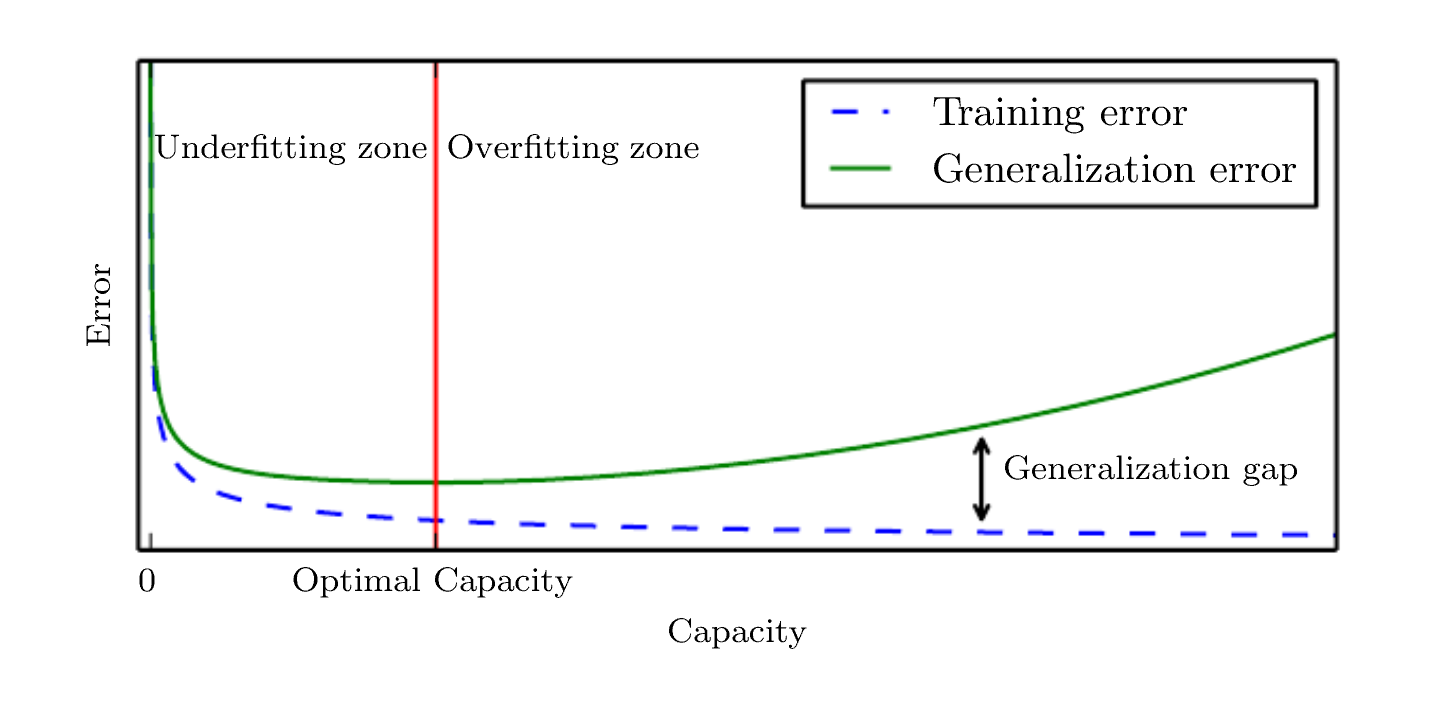
\includegraphics[width=\textwidth]{figures/MachineLearning3}
	\end{figure}


	There are three typical strategies for regularization, and we list them below:
		\begin{itemize}
			\item Put extra	constraints on a machine learning model: such as adding restrictions on the	parameter values.
			\item Add extra terms in the objective function that can be	thought of as corresponding to a soft constraint on the parameter values.
			\item Ensemble methods.
	\end{itemize}
	The	constraints and penalties for the first or second strategies usually have the properties list below:
			\begin{itemize}
				\item They are designed to encode specific kinds of prior knowledge.
				\item They are designed to express a generic preference for a simpler model class in order to promote generalization.
				\item They are necessary to make an underdetermined problem determined		 
			\end{itemize}
		
		\section{Parameter Norm Penalties}
		\subsection{Deep learning problem with penalty}
		The deep learning problem with penalty which we discussed in this section is 
		\begin{itemize}
			\item $\mathbb X = \{(\bm x^{(1)},y^{(1)}),...,(\bm x^{(m)},y^{(m)})\} \subset \mathbb R^n \times \mathbb R$ is a dataset. Let $\bm X =(\bm x^{(1)},...,\bm x^{(m)})$, $\bm Y=(y^{(1)},...,y^{(m)})$.
			\item Let $f:\mathbb R^n\rightarrow \mathbb R$ is the neural network function of $\bm x\in \mathbb R^n$, and has parameter $\bm w \in \mathbb R^p$, write as $f(\bm x;\bm w)$.
			\item $L(u,v):\mathbb R \times \mathbb R \rightarrow \mathbb R$ is the loss function. And
			$$
			\mathcal L(\bm u,\bm v)=\dfrac 1m\sum_{i=1}^m L(u_i,v_i)
			$$
			\item $J:\mathbb R^p\rightarrow \mathbb R$ is a function of $\bm w$ which describe the complexity of $f$. $\alpha$ is a constant. 
			\item Let $\bm F(\bm X;\bm w)=(f(\bm x^{(1)};\bm w),...,f(\bm x^{(m)};\bm w))$, $\mathcal{L}(\bm w) = \mathcal L(\bm F(\bm X;\bm w),\bm Y) $ and $\tilde{\mathcal L}(\bm w) = \mathcal L(\bm w) + \alpha J(\bm w) $\\ Solve:
			$$
			\bm \theta_{ML}=\arg \min_{\bm w}(\tilde{\mathcal L}(\bm w) )
			$$
	\end{itemize}


		
		\subsection{$L^2$ Parameter Regularization}
	
		
		One of the simplest and most common kinds of parameter norm penalty: the $L^2$ parameter norm penalty commonly known as \textbf{weight decay}:
		$$
		J(\bm w) = \dfrac{1}{2}||\bm w||_2^2
		$$
		
		In other academic communities, $L^2$ regularization is also known as \textbf{ridge regression} or \textbf{Tikhonov regularization}.
		
		$$
		\tilde{\mathcal{L}} (\bm w) = \dfrac{\alpha}{2} {\bm w}^T\bm w + \mathcal L(\bm F(\bm X;\bm w),\bm Y)
		$$
		$$
		\nabla_{\bm w}\tilde{\mathcal{L}} (\bm w) = \alpha\bm w + \nabla_{\bm w} \mathcal L(\bm F(\bm X;\bm w),\bm Y)
		$$
			To explain what happens over the entire course of training, we can consider the approximation of $\mathcal L$. Let
			$$
				\bm w^*= \text{arg} \min_{\bm w} \mathcal{L}(w)
			$$
			and $\hat{\mathcal{L}}$ is the approximation(2-order Taylor series) of $\mathcal L$ near the $\bm w*$, i.e. 
			$$
				\hat{\mathcal{L}} = \mathcal{L}(\bm w^*) + \dfrac{1}{2}(\bm w - \bm w^*)^T\bm H(\bm w - \bm w^*)
			$$
			where $\bm H$ is the Hessian matrix of $\mathcal{L}$. (Notice $\nabla_{\bm w}\mathcal{L}(\bm w^*)=0$.)
			Then the gradient of $\hat{\mathcal{L}}$ is 
			\begin{equation}\label{1}
				\nabla_{\bm w} \hat{\mathcal{L}} = \bm H(\bm w - \bm w^*)
			\end{equation}
				
			To study the effect of weight decay, we modify equation \eqref{1} by adding the
			weight decay gradient. We can now solve for the minimum of the regularized
			version of $\hat{\mathcal{L}}$. We use the variable $\tilde{\bm w}$ to represent the location of the minimum.
			$$
			\alpha \tilde{\bm w} + \bm H(\tilde{\bm w} - \bm w^*)=0
			$$
			Then we can get
			\begin{equation}\label{2}
				\tilde{\bm w} = (\bm H + \alpha \bm I)^{-1}\bm H \bm w^*
			\end{equation}
			
			where $\bm I$ is the identity matrix.
	
			As $\alpha \rightarrow 0$, $\tilde{\bm w}\rightarrow \bm w^*$, but what happens as $\alpha$ grows? Because	$\bm H$	is real and symmetric, then we have eigenvalue decomposition:
			$$ \bm H = \bm Q^T \bm \Lambda \bm Q$$
			Applying the decomposition to equation \eqref{2}, we obtain:
			$$
			\tilde{\bm w} = \bm Q(\bm \Lambda +\alpha \bm I)^{-1}\bm \Lambda \bm Q^T \bm w^*
			$$
			We see that the effect of weight decay is to rescale $\bm w^*$ along the axes defined by the eigenvectors of $\bm H$. Specifically, the component of
			$\bm w^*$ that is aligned with the $i$-th eigenvector of $\bm H$ is rescaled by a factor of	$\dfrac{\lambda_i}{\lambda_i+\alpha}$. It's the same as Tikhonov regularization in inverse problem theory.
		\subsection{$L^1$ Regularization}
		Formally, $L^1$	regularization on the model parameter w is defined as
		$$
		J(\bm w) = ||\bm w||_1 = \sum_i|w_i|
		$$
		and
		$$
		\tilde{\mathcal{L}}(\bm w) =\alpha ||\bm w||_1 + \mathcal L(\bm F(\bm X;\bm w),\bm Y)
		$$
		with gradient:
		$$
		\nabla_{\bm w}\tilde{\mathcal{L}}(\bm w) =\alpha \text{sgn}(\bm w) + \nabla_{\bm w} \mathcal L(\bm F(\bm X;\bm w),\bm Y)
		$$
			Because the $L^1$ penalty does not admit clean algebraic expressions in the case
			of a fully general Hessian, we will also make the further simplifying assumption
			that the Hessian is diagonal, $\bm H =\text{diag}(H_{1,1},\cdots,H_{n,n})$, where $H_{i,i}>0$.
			
			Then we have 			
			$$
			\hat{\mathcal{L}} = \mathcal{L}(\bm w^*) +\sum_i \dfrac{1}{2}H_{i,i}(w_i - w_i^*)^2
			$$
			when can get the
			$$
			\tilde w_i =\text{sign}(w_i^*)\max \{|w_i^*|-\dfrac{\alpha}{H_{i,i}},0 \}
			$$
		Consider the situation where $w^*_i>0$ for all $i$. There are two possible outcomes:
			\begin{itemize}
				\item The case where $ w^*_i\leq\dfrac{\alpha}{H_{i,i}}$, then $\tilde{w}_i=0$.  This occurs because the contribution of $\mathcal{L}$ to the regularized objective $\tilde{\mathcal L}$ is overwhelmed--in direction $i$--by the $L^1$ regularization which pushes the value of $w_i$ to zero.
				
				\item The case where $ w^*_i >\dfrac{\alpha}{H_{i,i}}$.  In this case, the regularization does not move the optimal value of $w_i$ to zero but instead it just shifts it in that direction by a distance equal to $\dfrac{\alpha}{H_{i,i}}$
			\end{itemize}
			A similar process happens when $w^*_i<0$.
			In comparison to $L^2$ regularization, $L^1$ regularization results in a solution that is more sparse.
	
	\section{Ensemble Methods}
	\subsection{Dataset Augmentation}
		The best way to make a machine learning model generalize better is to train it on
	more data. Of course, in practice, the amount of data we have is limited. One way
	to get around this problem is to create fake data and add it to the training set.
	For some machine learning tasks, it is reasonably straightforward to create new
	fake data.
	
	This approach is easiest for classification. A classifier needs to take a complicated, high dimensional input $\bm x$ and summarize it with a single category identity $y$. This means that the main task facing a classifier is to be invariant to a wide variety of transformations. We can generate new $(\bm x, y)$ pairs easily just by transforming
	the $\bm x$ inputs in our training set. But this approach is not as readily applicable to many other tasks.

	\subsection{Bagging and Other Ensemble Methods}
		\begin{itemize}
			\item \textbf{Bootstrap} comes from a common saying "pull up by your own bootstraps", which means use your won resource to solve problem.
			\item \textbf{Bagging} (short for \textbf{bootstrap aggregating}) is a technique for reducing generalization error by combining several models. The idea is to train several different models separately, then have all of the models vote on the	output for test examples.This is an example of a general strategy in machine learning called	model averaging. Techniques employing this strategy are known as ensemble methods.
			\item The reason that model averaging works is that different models will usually
			not make all the same errors on the test set.
		\end{itemize}
		Neural networks reach a wide enough variety of solution points that they can often benefit from model averaging even if all of the models are trained on the same dataset. Differences in random initialization, random selection of minibatches,
		differences in hyperparameters, or different outcomes of non-deterministic implementations of neural networks are often enough to cause different members of the ensemble to make partially independent errors.
	\subsection{Dropout}
			 \textbf{Dropout} provides a computationally inexpensive but	powerful method of regularizing a broad family of models. To a first approximation, dropout can be thought of as a method of making bagging practical for ensembles of very many large neural networks. Specifically, dropout trains the ensemble consisting of all sub-networks that can be formed by removing non-output units from an underlying base network.
		
		\newpage
		\begin{figure}
			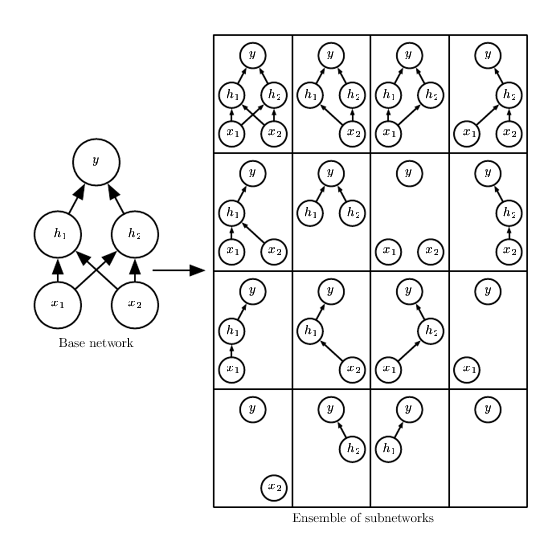
\includegraphics[width=\linewidth]{figures/dropout}
			\caption{Dropout trains an ensemble consisting of all sub-networks that can be
				constructed by removing non-output units from an underlying base network.}
			\label{fig:dropout}
		\end{figure}

		\begin{wrapfigure}{r}{0.4\textwidth}
			\vspace{-20pt}
			\begin{center}
				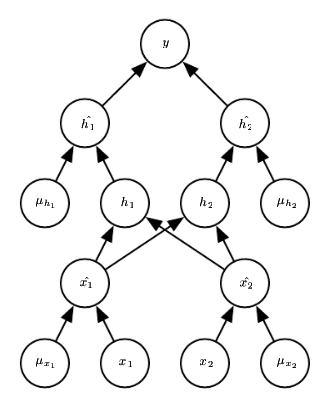
\includegraphics[width=0.38\textwidth]{figures/dropoutexample}\label{dropoutexample}
			\end{center}
			\vspace{-20pt}
			\vspace{-10pt}
		\end{wrapfigure}
		
		To perform forward propagation with dropout, we randomly sample a vector $\bm \mu$ with one entry for each input
		or hidden unit in the network. The entries of $\bm \mu$ are binary and are sampled independently from each other. The probability of each entry being 1 is a hyperparameter, usually $0.5$ for the hidden layers and $0.8$ for the input. Each unit in the network is multiplied by the corresponding mask, and then forward propagation continues through the rest of the	network as usual. This is equivalent to randomly selecting one of the sub-networks from figure and running forward propagation through it.
	
		 Recall that to learn with bagging, we define $k$ different models, construct $k$ different datasets by sampling from the training set with replacement, and then train model $i$ on dataset $i$. Dropout aims to approximate this process, but with an exponentially large number of neural networks. Specifically, to train with dropout, we use a minibatch-based learning algorithm that makes small steps, such as stochastic gradient descent. Each time we load an example into a minibatch, we randomly sample a different binary mask to apply to all of the input and hidden units in the network. 

		Dropout training is not quite the same as bagging training. In the case of
		bagging, the models are all independent. In the case of dropout, the models share
		parameters, with each model inheriting a different subset of parameters from the
		parent neural network. This parameter sharing makes it possible to represent an
		exponential number of models with a tractable amount of memory. In the case of
		bagging, each model is trained to convergence on its respective training set. In the
		case of dropout, typically most models are not explicitly trained at all—usually,
		the model is large enough that it would be infeasible to sample all possible sub-
		networks within the lifetime of the universe. Instead, a tiny fraction of the possible
		sub-networks are each trained for a single step, and the parameter sharing causes
		the remaining sub-networks to arrive at good settings of the parameters. These
		are the only differences. Beyond these, dropout follows the bagging algorithm.

	
\end{document}